\documentclass{../src/bcthesispart}
\title{Numeral systems}
\author{Bas Cornelissen}
\begin{document}
%——————————————————————————————————————————————————————————
\parttitle{Numeral systems}%
	{Numeral systems}%
	{numerals}%
	{% Abstract
	Models of cultural language evolution are seen to be ecologically valid, primarily because their conclusions are reproducible in equivalent laboratory experiments.
	More direct comparisons seem vital, and this chapter proposes numeral systems as a test case.
	Various reasons are given: reconstructions of their development have been proposed, lots of empirical data are available, the design space is vast, cognitive mechanisms well-studied and finally, numerals are simple enough to be easily modelled.
	The next chapter addresses early attempts at modelling the cultural evolution of numeral systems.
	}
%——————————————————————————————————————————————————————————



\noindent
Numerals, as Bernard Comrie once put it, seem to be one of the rare cases where “present-day languages provide direct insight into the evolution of language” \parencite{Comrie2013}.
They suggest an evolution in multiple stages, starting with words for the  numbers 1--4, then building up a counting sequence, which gave rise to ‘serialised’ additive constructions and finally to the fully recursive systems that prevail today.
He was not the first to note this.
The multistage evolution of numerals was one of the central ideas developed in James Hurford’s \emph{Language and Number}.
Numeral systems, he writes “show marks of successive phases of invention in the building up of the whole.” (p.~78).
As a result, “one can ‘read’ the history of a system, just like the history of an old building, from the contrasting styles of its pieces, from the foundations up” (p.\ 83).
If it possible to reconstruct the evolution of numeral systems, doesn’t that make it the ideal test case for models of language evolution?
That is exactly what I suggest in this chapter.
%%



%——————————————————————————————————————————————————————————
%——————————————————————————————————————————————————————————
\section{Balancing expressivity and simplicity}
%——————————————————————————————————————————————————————————
%——————————————————————————————————————————————————————————



A good empirical test case is indispensable. 
As \textcite{Dediu2013} observe, “much work in agent-based modelling has proceeded in the absence of empirical linguistic data, input from linguists, or psychological considerations regarding learning, memory and processing” (p.~ 330).
The absence might be a side effect of a growing body of laboratory experiments with cultural evolution (see \textcite{Tamariz2017} for a recent review), providing evidence for the ecological validity of the models \parencite{Smith2014}.
To give one famous example, \textcite{Kirby2008} presented human participants, organised in a transmission chain, with an artificial language learning task.
The first participant learned randomly generated names for a subset of a larger collection objects, which differed in colour, shape and movement.
In a testing phase, the subject was asked to reproduce the names of \emph{all} the objects, including unseen ones.
A subset of the reproduced names was used to train the next subject.
That subect again reproduced names for all objects, which were presented to another subject, and so on.
Transmitting only a subset of the meaning-symbol pairs gave rise to a transmission bottleneck.
This led to increase in learnability in the form of a systematic underspecification.
The resulting language for example only distinguishes shape, but ignores colour and movement.
Underspecification comes at the cost of expressivity, but when adding a pressure for expressivity, compositional languages emerged (see figure \ref{fig:ch5:kirby}).
Initially, this pressure was imposed by artificially removing homonymy \parencite{Kirby2008}, later by introducing communication in a chain of dyads \parencite{Kirby2015}.
In either case, the experimental findings are surprisingly consistent with early iterated learning models and are therefore said to “provide empirical support for computational and mathematical models of iterated learning” \parencite{Kirby2008}.
%%


%- - - - - - - -
\begin{SCfigure}
	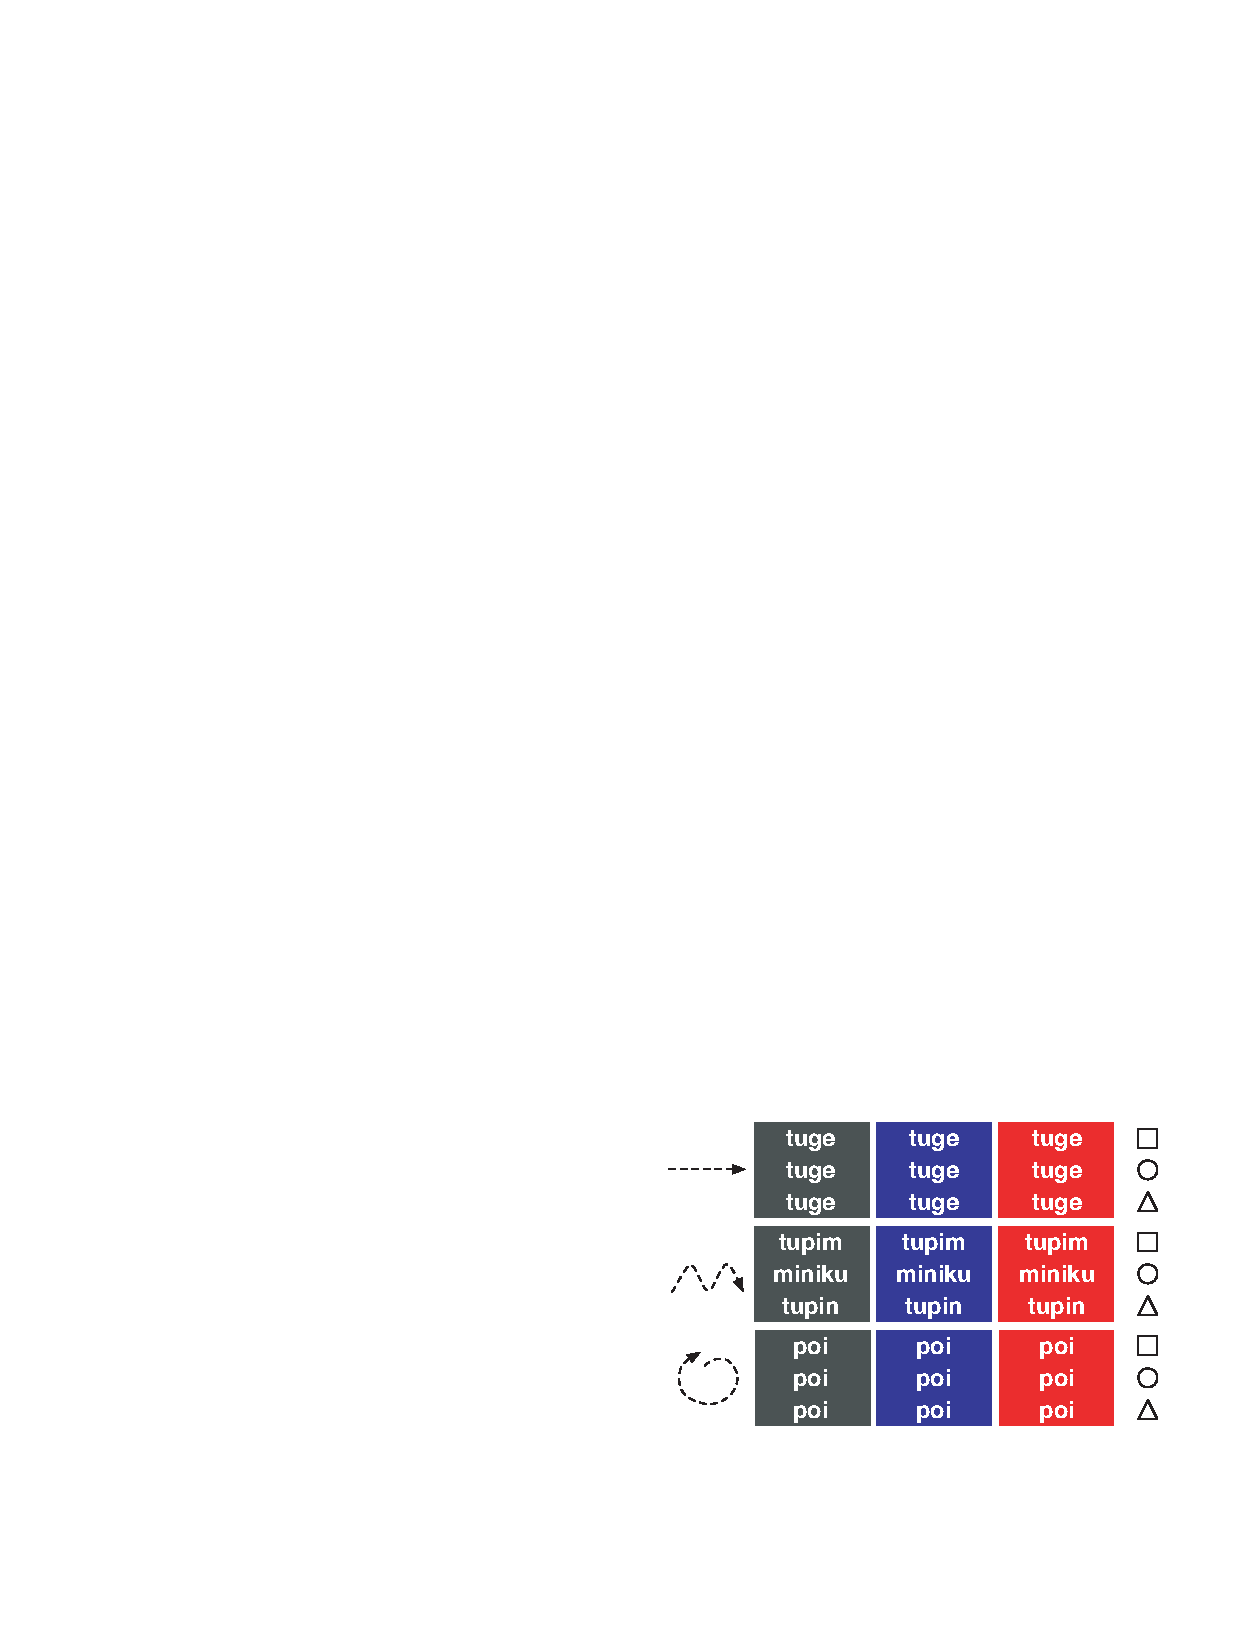
\includegraphics[width=.45\textwidth]{../figures/CH5-kirby2008-fig1}
	\hfill
	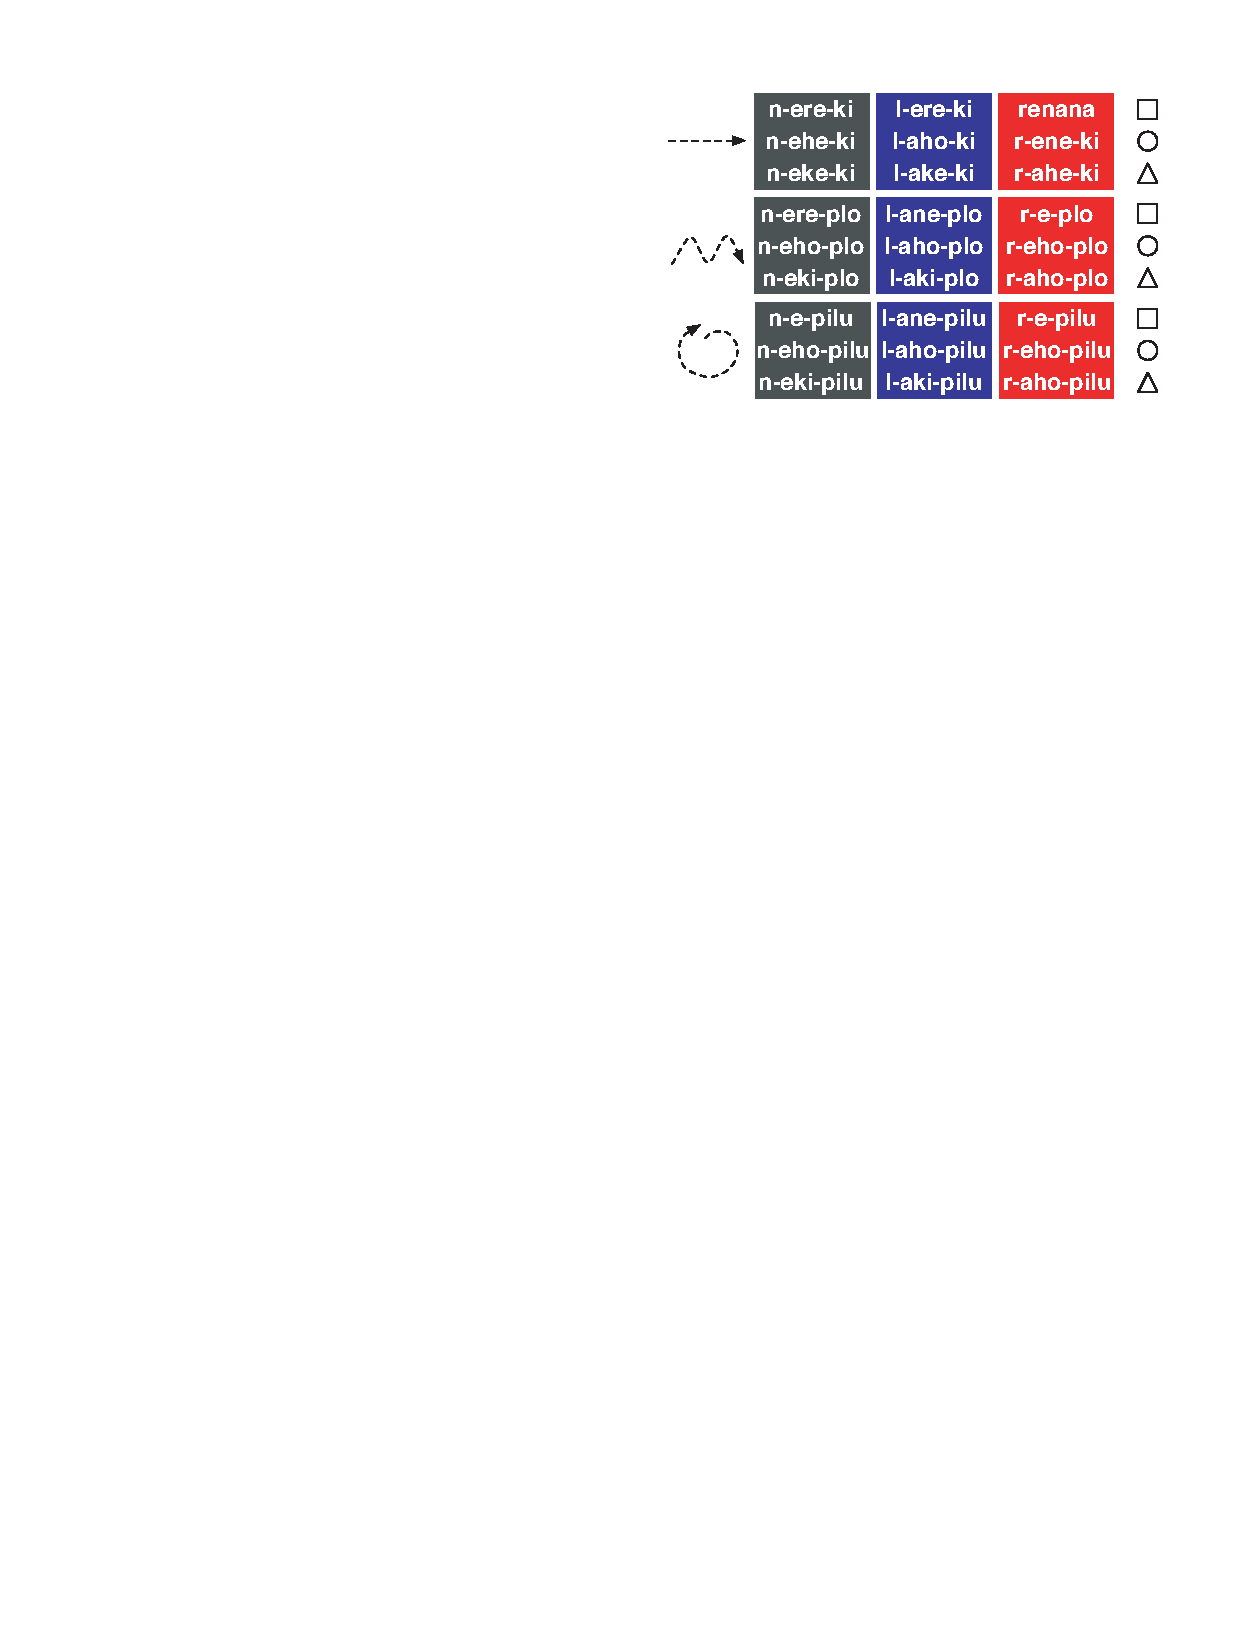
\includegraphics[width=.45\textwidth]{../figures/CH5-kirby2008-fig2}
	%---------
	\caption{Transmission pressures for learnable languages, resulting in systematic underspecification (left). 
	Introducing a pressure for expressivity results in compositional structure (right).
	%----------
	\figdetails{Figure reproduced from \textcite{Kirby2008} without permission.
	\label{fig:ch5:kirby}}}
	%todo (optional) add subfigure titles
\end{SCfigure}
%- - - - - - -



The idea that language balances competing pressures for expressivity and learnability connects iterated learning to the work of Terry Regier and colleagues.
In a series of papers, they argue that languages are optimised for efficient communication, implying a similar balance between expressivity and simplicity.
They found evidence for this in colours terms \parencite{Regier2007}, kinship relations \parencite{Kemp2012}, spatial relations \parencite{Khetarpal2013,Regier2015}, and, indeed, numeral systems \parencite{Xu2014}.
It was soon recognised that iterated learning might explain the observed near-optimality \parencite{Levinson2012}.
\textcite{Xu2010} and \textcite{Carstensen2015} accordingly set up iterated learning experiments where human subjects reproduced colour terms, concluding that “colour-naming universals may come from the learning and perceptual biases of human learners, brought out through the process of cultural transmission” \parencite{Xu2010}.
Interestingly, perceptual biases in the form of just-noticeable differences, were also sufficient to reproduce realistic colour-term patterns in a simulation using a variant of the naming game \parencite{Baronchelli2010}. 
%%



However, colour terms might not provide the most convincing case for the argument that \emph{compositional} structure in language results from pressures for learnability and expressivity \parencite[e.g.][]{Kirby2015} — colour terms have, to the best of my knowledge, typically no compositional structure.
In that respect numeral system are much more promising. 
Few, if any, structures seem to balance expressivity and simplicity so effectively
Most languages can accurately name a vast range of numbers using a small lexicon and some simple recursive rules. 
In English, for example, the thirteen words \lng{one}, \lng{two}, \lng{three}, \lng{four}, \lng{five}, \lng{six}, \lng{seven}, \lng{eight}, \lng{nine}, \lng{ten}, \lng{hundred}, \lng{thousand}, and \lng{million} can be used to name nearly all numbers up to one billion ($10^9$). 
This might make numerals atypical linguistic structures, but that does not mean their structure cannot be explained by typical linguistic processes such as grammaticalisation \parencite{VonMengden2008}.
%%




This chapter, then, has two goals.
First, it argues that numeral systems are a good test case for models of language evolution.
One argument can be found in the discussion above — numerals balance simplicity and expressivity, which should be reproducible using iterated learning — and further arguments are developed later in this chapter.
Second, the chapter outlines the basic structure of numeral systems, a prerequisite for all that follows.
In light of the above discussion, the \emph{internal}, arithmetical structure of numerals is of primary interest and not, say, the grammatical role of numerals (e.g.~why is \lng{five blue balls} grammatical, and \lng{blue five balls} not?).
Restrictions of this type are necessary, since the linguistic literature on numerals is vast.
In one survey, Harald Hammerström identifies 13 500 references to primary sources, over 100 monographs and hundreds of articles. 
I am practically oblivious to all this literature and will rely on several more general, secondary sources, which fortunately sketch a relatively clear picture of the world’s numeral systems.
	\nocite{Hurford1975, Hurford1987, Greenberg1978, Hammarstrom2009, Comrie2013, Hanke2010, VonMengden2008}
%%





%——————————————————————————————————————————————————————————
%——————————————————————————————————————————————————————————
\section{An introduction to numeral systems}
%——————————————————————————————————————————————————————————
%——————————————————————————————————————————————————————————


%——————————————————————————————————————————————————————————
\paragraph{Defining numerals}

So what exactly are numerals? 
Numerals are expressions for numbers, but we need to be more preicse.
The the expressions of interest are \emph{cardinals} like \lng{one, two, three}.
These express quantity and should should be distinguished from \emph{ordinals} such as \lng{first, second, third} expressing order.
\textcite{VonMengden2008} presents a categorisation that clearly distinguishes cardinals from other quantifiers; it is reproduced in figure \ref{fig:ch5:quantifiers}.
At the highest level he distinguishes \emph{numerically specific} from numerically \emph{unspecific} quantifiers. The latter include vague quantifiers such as \lng{some} and \lng{many} but also universals such as \lng{all}.
Other words, like \emph{score} and \emph{dozen} have specific muneric values, but are typically not considered to be numerals, for the simple reason they are not part of a \emph{system} in they way \lng{one, two, three,} and so on, are. 
They for instance do not normally occur in the counting sequence. 
%%




%- - - - - - - -
\begin{SCfigure}
	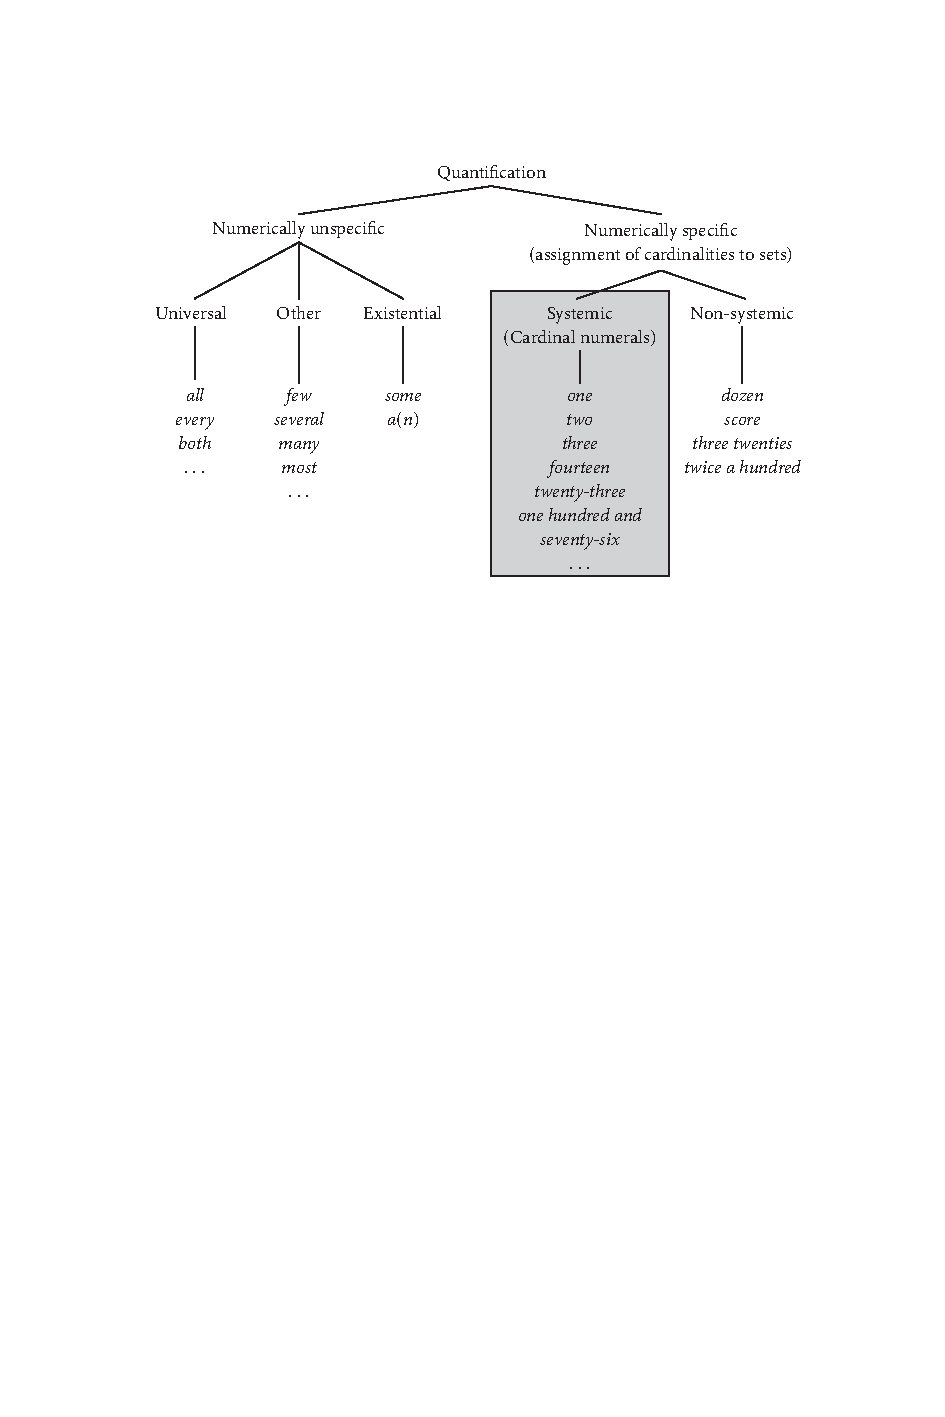
\includegraphics{../figures/CH5-quantifiers}
	\caption{Numerals are numerically specific, systematic quantifiers.
	%----------
	\figdetails{Reproduced from \textcite{VonMengden2008} without permission.}
	\label{fig:ch5:quantifiers}}
\end{SCfigure}
%- - - - - - -




To a first approximation, numerals are systematic, numerically specific expressions, but considering a more refined definition is instructive.
\textcite{Hammarstrom2009} defines numerals as
“(1) spoken, 
(2) normed expressions that are used to denote the 
(3) exact number of objects for an 
(4) open class of objects in an 
(5) open class of social situations with 
(6) the whole speech community.”
These clauses exclude certain other numerical expressions. 
Symbolic systems such as Roman and Arabic number symbols are excluded by (1); non-standard expressions like \lng{three-times-five-and-two} for \lng{seventeen} are excluded by (2); and 
(3) excludes numerically unspecific expressions.
(4) excludes counting systems that are exclusively used to count a restricted class of objects, such as the Wuvulu system for counting coconuts \parencite{Hammarstrom2009}.
(6) excludes specialised (mathematical or technical) jargon, and (5) excludes body-tally systems.
Those systems use a fixed sequence of body parts to which speakers point when indicating a number.
The sequences can be quite elaborate: some extended body counting systems in the highlands of New Guinea use a sequence of 23 body parts\footnote{%
	%>>>
	Starting on the left side of the body: little finger, ring finger, middle finger, index finger, thumb, wrist, middle of forearm, inside of elbow, middle of upper arm, shoulder, collarbone, hole above breastbone, and then continuing in reverse order at the other side of the body
	%<<<
	} \parencite{Comrie2013}.
As Hammerström explains, “body tallying has to be done on a physically present person and to understand what number is referred to, the process must be watched”.
This makes body-tally systems markedly different from the other numeral systems.
%%




The constraints (1)--(6) can hardly be called restrictive. 
\textcite{Hammarstrom2009} estimates there are at least 3500 numeral systems. Accordingly, Numeralbank,\footnote{%
	%>>>
	Numeralbank is part of Glottobank and largely based on the work of Eugene Chan. 
	He collected many numeral systems at \href{https://mpi-lingweb.shh.mpg.de/numeral/}{mpi-lingweb.shh.mpg.de/numeral}{}. 
	For most languages, it contains the expressions for 1--30, 40, 50, 60, 70, 80, 90, 100, 200, 1000 and 2000.
	%<<<
	}
a databank of numeral systems, contains around 4200 numeral systems. 
These numeral systems can be divided in at least two categories: \emph{restricted} and \emph{recursive systems} \textcite{Comrie2011,Xu2014}.
Restricted systems have little internal structure (e.g.\ all numbers are lexicalised or use only additive constructions) and typically cannot express numbers higher than 20. 
These systems are extremely rare. 
Most numeral systems are recursive, meaning they are organised around one or several bases and use multiplication and addition to recursively express a vast range of numbers.
English uses the bases 10, 100 and 1000 (and possibly more), and happens to be a representative example: 
The vast majority of the world’s languages use a decimal system, followed by vigesimal (base 20) and quinary (base 5) systems \parencite{Comrie2013}.
Yet many other systems exist. 
There are languages without base, or languages using base 3, 4, 5, 6, 8, 12 or 15, perhaps supplemented by higher bases like 40, 60 and 80 \parencite[see][for a survey]{Hammarstrom2009}.
%%




%——————————————————————————————————————————————————————————
\paragraph{Simple numerals, complex numerals and bases}

Let’s spell out the structure of numeral systems in more detail, by considering the English system. 
The first ten numbers are expressed by mono-morphemic forms which we will call \emph{simple numerals} \parencite{VonMengden2008}.
Forms like \lng{hundred} or \lng{thousand} are also simple numerals.
They can be combined to form \emph{complex numerals} such as \lng{two thousand three hundred sixty five}.
The transition between simple and complex numerals can be a smooth one, as evident from French: \lng{onze (11), douze (12), treize (13), quatorze (14), quinze (15), seize (16), dix-sept (17), dix-huit (18), dix-neuf (19)} \parencite{Calude2016}.
Simple numerals can be further subdivided in \emph{atoms} and \emph{bases}. 
The atoms are the numerals from \lng{one} up to \lng{nine}; \lng{ten, hundred} and \lng{thousand} are the bases (higher bases are discussed later).
Even if bases are “the most salient single characteristic” of numeral systems \parencite{Hammarstrom2009}, defining what exactly counts as a base is tricky. 
%%



\textcite{Comrie2013} defines a base as a number $b$ occurring in multiplicative expressions of the form $x \times b + y$, where he stresses that order is unimportant.
Although the idea is clear, it is not precise enough:
The expression \lng{six hundred and four} is of the given form, but should not suggest that $6$ is an English base. 
\textcite{Greenberg1978} opts for a more technical definition.
From a linguistic point of view, $2\times 10$ (\lng{two tens}) and $10\times 2$ (\lng{ten twos}) are not identical.
The order of the factors indicates which of the two is the `constant' (\emph{augend} in additive/\emph{multiplicand} in multiplicative constructions) and which the `variable' (\emph{addend}/\emph{multiplier}). 
Bases, according to Greenberg, are multiplicands occurring in a series like $2 \times 10, 3\times 10, 4\times 10, \dots$ — they are \emph{serialised multiplicands}.
But even this definition has shortcomings: 
It ignores subtractive constructions of the form $x \times b - y$.
\textcite{Hammarstrom2009} \emph{does} account for those and defines a number $b_i$ to be a base if 
(1) the next higher base $b_{i+1}$ is a multiple of $b_i$ and 
(2) “a proper majority” of the numbers between $b_i$ and $b_{i+1}$ are expressed as $n\times b_i + k$ or $n \times b_i - k$ for some $k < b_i$. 
For English, this definition designates $10$, $100$, $1000$, $10^6$ and $10^9$ as bases. 
Indeed, definitions are difficult, but the idea should be clear.
%%




%——————————————————————————————————————————————————————————
\paragraph{Isolated, mixed and additive bases}

It will be convenient to introduce some terminology for ‘special’ base-like numbers, that are not bases in the strict sense.
French is famous for containing remnants of a vigesimal system, expressing numbers above 80 using base 20, as in \inlgloss{quatre-vingt-dix-sept}{four-twenty-ten-seven}{$97=4 \times 20 + 10 + 7$}.
However, using Hammarström’s definition, this would not make 20 a French base, as only a minority of the numbers between 20 and 100 (the next base) are expressed using 20. 
\textcite{Comrie2011} calls such cases \emph{isolated} bases.
%%



The Welsh expression \inlgloss{deu naw}{two nine}{$18=2 \times 9$} is another example of an isolated base, since Welsh has a fairly clear vigesimal system — with one notable exception:
It uses 100 as a base, which is not a power of 20. 
When the bases in a system are not powers of a single base, the system has \emph{mixed bases}. 
In the case of Welsh, 20 does qualify as a base, since most numbers between 20 and 99 are expressed using multiples of 20. 
70 is for example expressed as \inlgloss{deg a thrigain}{ten on three-twenty}{$3\times 10$}. 
Such mixed vigesimal-decimal system are very common \parencite{Comrie2013}, but other mixes are also attested. 
Supyire uses a particularly complex mix of base 20, 80 and 400, while expressing numbers below 20 using additive constructions involving 5 and 10. 
\textcite{Comrie2011} gives the expression for 799 as
%~~
\begin{exe}
	\ex\gll%
	kàmpwóò ŋ̀kwuu sicyɛɛré 'ná béé-tàànre ná kɛ́ 'ná báár-ìcyɛ̀ɛ̀rè\\
	fourhundred eighty four and twenty-three and ten and five-four\\
	\hfill Supyire
	\glt $799=400 + (80 \times 4) + (20 \times 3) + 10 + (5 + 4)$
\end{exe}
%~~
%%




Additive constructions for numbers below the lowest base, as with 10 and 5 in Supyire, occur in more languages. 
Mixtec languages for example use a vigesimal system with single words for 10 and 15.
%todo (optional) include a table with Mixtec numerals?
The same pattern is found in Biblical Welsh \parencite{Hurford1975}.
Georgian expresses the number 11 to 19 using addition with 10, which is reminiscent of the French \lng{quatre vingt dix sept}, where 10 is used in a similar additive construction. 
In these examples, 5, 10 or 15 are not proper bases, but one might call such numbers \emph{additive bases}, if they are smaller than the first base and occur in multiple additive constructions — that is, if they are \emph{serialized augends} \parencite{Greenberg1978}.
It should be stressed that neither additive nor isolated bases are bases according to Hammerström’s definition, while mixed bases are.
%%




%——————————————————————————————————————————————————————————
\paragraph{Exponentiation and mathematical bases.}

The notion of ‘base’ is used in mathematics, in a similar, but different way.
A decimal system in the mathematical sense uses bases $10^0, 10^1, 10^2, 10^3, 10^4, 10^5, \dots $, whereas a decimal system in the linguistic sense would use a finite subset such as $10^2, 10^3, 10^6, 10^9$.
The defining property of mathematical bases is that they are exponents.
It has been argued that exponentiation also plays a defining role in numeral systems \parencite[e.g.][]{Hurford1975}, but this is controversial \parencite[see][]{Comrie1999,Comrie2013}. 
First, nothing signals that \lng{hundred} and \lng{thousand} correspond to the first and second power of 10.
The use of portmanteau forms for high bases is in fact widespread: \lng{million} originates from Italian \lng{millione}, the augmentative of \lng{mille} (thousand), something like ‘a big thousand.’
Second, even if the sequence \lng{billion}, \lng{trillion}, \lng{quadrillion}, and so on, is somewhat productive, the relation to the corresponding powers is opaque ($n$-illion meaning $10^{3n+3}$). 
Third, such high powers are, with the notable exception of at least Sanskrit (see below), often a recent invention used mostly in technical context. 
Finally, exponentiation is not very consistent across languages.
Illustrating the last few points, the UK adopted the so called \emph{short scale system} in favour of the \emph{long scale system} as recently as 1974.
The short scale system uses \lng{million} for $10^6$, \lng{billion} for $10^9$, \lng{trillion} for $10^{12}$, and so on; the long scale system uses \lng{million} for $10^6$, \lng{milliard} for $10^9$, \lng{billion} for $10^{12}$, \lng{billiard} for $10^{15}$, and so on. 
Mandarin uses a completely different sequence of powers: $10^4$, $10^8$, $10^{12}$, $10^{16}$.
Sanskrit even has a monomorphemic series of bases for all powers of 10 up to $10^{11}$ \parencite{Comrie2011}.
The simple and safe solution, in sum, is to define the bases of a numeral system by listing all of them.
%%




%——————————————————————————————————————————————————————————
\paragraph{Subtraction, division and fractions}

Arithmetical operations other than addition and multiplication are also used. One finds subtraction in the Latin expression \inlgloss{un-de-viginti}{one-from-twenty}{$19=20\leftarrow 1$}, where I wrote $a \leftarrow b$ for $b-a$ to respect the order of the constituents.
In Biblical Welsh, one finds expressions like \inlgloss{onid pedwar deugain}{minus four two-twenty}{$36 = -4 + 2 \times 20$} and Ket expresses 70, 80 and 90 as $100-30$, $100-20$, $100-10$ respectively.
\textcite{Comrie2011} gives the example
%~~
\begin{exe}
	\ex\gll%
	qus’am ʌɣam dɔŋas’ bən’s’aŋ ²kiʔ\\
	one left.over thirty without hundred 
	\\\hfill Ket
	\glt $71 = 1 + (30 \leftarrow 100)$
\end{exe}
%~~
%%




Some languages even use division, although it might be more accurate to speak of multiplication by fractions \parencite{Comrie2011}.
Welsh expresses 50 as \inlgloss{half cant}{half hundred}{$50=\nicefrac{1}{2} \times 100$}. 
Danish offers more examples, expressing 50 as \inlgloss{halvtreds}{}{}, which is derived from \inlgloss{halv-tred-sinds-tyve}{half-third-times-twenty}{$50 = 2 \nicefrac{1}{2} \times 20$}. 
Here half-third can be interpreted as the third half: $2 \nicefrac{1}{2}$ after $\nicefrac{1}{2}$ and $1 \nicefrac{1}{2}$, but \textcite{Comrie2011} lists it as an example of \emph{overcounting}.
%%




%——————————————————————————————————————————————————————————
\paragraph{Overcounting and overrunning.}

The English equivalent of overcounting would be the expression\inlgloss{three on the way to to fifty}{}{} for 43. 
More formally, if $b$ is some base, an example of overcounting is of the form \lng{$a$ towards $(x+1) \times b$} for $x\times b + a$. 
One could read an example of overcounting in \lng{half-tred}: 
half on the way to three, but the interpretation ‘the third half’ also seems likely. 
Clearer examples are cited by Hurford (1975). 
Some Mayan languages express 41 as \lng{huntuyoxkal}, which translates to \lng{the first of the third score} ($1+ 3\times 20$). 
\emph{Overrunning} is a different phenomenon, where one uses addition when multiplication might be expected, or multiplication if a higher base would be expected. 
The English equivalent would be \lng{tenteen} for 20 or \lng{tenty} for 100. 
Comrie (1992) gives several examples, starting with Polabian
%~~
\begin{exe}
	\ex\glll%
	visem-nocti, diva(t)-nocti, disa(t)-nocti\\
	eight-ten, nine-ten, ten-ten\\
	18, 19, 20\\
	\hfill Polabian
\end{exe}
%~~
The French \lng{soixante dix neuf} ($6 \times 10 + 10 + 9$) would be another example, and indeed some varieties of French have adopted the simpler \lng{septante neuf}. 
A clear example of multiplicative overrunning can be found in Old Islandic
%~~
\begin{exe}
	\ex\glll%
	{otto tiger}, {níu tiger}, {tío tiger}, {ellefo tiger}\\
	{eight ten}, {nine ten}, {ten ten}, {eleven ten}\\
	{$8\times 10$}, {$9 \times 10$}, {$10\times 10$}, {$11\times 10$}\\
	\hfill Old Islandic
\end{exe}
%~~
%%




%——————————————————————————————————————————————————————————
\paragraph{order}

Languages can differ in how they order the constituents of numerals.
The English \inlgloss{twenty five}{}{$20+5$} becomes \inlgloss{vijfentwintig}{five-and-twenty}{$5+20$} in Dutch, and German similarly ‘reverses’ the order.
As \textcite{Calude2016} point out, the ordering (base--atom, as in English or atom--base as in Dutch) has not always received enough attention.
But there are interesting regularities.
If languages use both the base--atom and atom--base order, the system always uses atom--base for the smallest numbers and at some point switches to base--atom. The reverse never happens \parencite{Greenberg1978}.
Greenberg proposed the cognitive explanation that for large numbers the base term is much more informative and salient.
\textcite{Calude2016} find that in Indo-European languages, the change in order, if it happens, practically always happens below 20.
%%





%——————————————————————————————————————————————————————————
\paragraph{Continuity of the counting sequence}

Another property of numeral systems is that they never have gaps.\footnote{%
	%>>>
	But see \textcite{Zhou2015} for \emph{possible} gaps in some \emph{restricted} Australian systems.
	%<<<
	}
If a system can express numbers up to $L$, it has expressions for \emph{all} numbers $1, \dots, L$.
This perhaps unsurprising observation has some importance for philosophical discussions concerning the nature of numbers.
\textcite{Hurford1987} dedicates a full chapter to three possible explanations of the continuity.
First, in extreme form, the \emph{referential-pragmatic hypothesis} holds that cardinalities are properties of collections (‘threeness’) that are fairly directly perceptible (\emph{subitised}, see below).
Continuity follows from the claim that $n$ is more likely to be expressed than $n+1$. 
Second, the \emph{conceptual-verbal hypothesis} assumes we are born with the concepts \textsc{one}, \textsc{number} and \textsc{successor}.
As a result children cannot but construct a continuous sequence, like “little Peano’s.”
Third, the \emph{ritual hypothesis} assumes numbers are the result of reciting a ritualised sequence; the meaning is grounded in the ritual of counting.
All of these positions are problematic and Hurford therefore suggests a synthesis: Small numbers up to 3--4 are subitised and we learn the notion of successor only after exposure to a conventional counting sequence.
%%





%——————————————————————————————————————————————————————————
\paragraph{The packing strategy}

The main (near-)universal property of numeral systems formulated in \textcite{Hurford1975} is the so called \emph{packing strategy}.
Conceptually, it is a simple principle: “When forming an expression for a high number, pick the highest-valued expression available as a starting point, and then build on that” \parencite[243]{Hurford1987}. 
Even though it is regularly cited it has not received much attention in the literature.
One reason might be that the packing strategy was originally formulated as a fairly technical set of constraints on a phrase-structure grammar. 
But it is in fact a simple principle, \emph{both} technically and conceptually.
That becomes clear if you reformulate the principle \emph{outside} the specific framework of \textcite{Hurford1975}.
In appendix \ref{app:packing-strategy} I reduce the packing strategy to the claim that \emph{complex numerals use the largest multiple of the largest base possible.}
A slightly more general formulation would be \emph{the difference between $a$ and $b$ in $a+b$ and $a\times b$ should be maximised.}
For example, Mixtec uses both 15 and 10 as base and could thus express 19 as either $10 + 9$ or $15+4$. 
The packing strategy correctly picks the latter, as it uses the larger of the two possible bases 10 and 15.
Counterexamples also exist: \lng{twenty-three hundred} does \emph{not} conform to the packing strategy since \lng{two thousand three hundred} expresses the same number using a larger base.





%——————————————————————————————————————————————————————————
\paragraph{A decimal world}

The previous discussion should not suggest a world where any two languages will use a radically different numeral systems, with mixes of subtraction, overcounting, division, overrunning and what not.
No, that is certainly false.
In fact, “we live in a decimal world. 
[…] Bases other than 10 or 20 are extremely rare in the modern world” \parencite{Comrie2013}.
It is no big mystery why the particular base 10 is so prevalent — “no contemporary linguist has ever thought it necessary to spell this explanation out, let alone argue against it” (p.\ 39–40).
Indeed, boydy parts are a common source for certain number names: “Nouns for ‘hand’ probably provide the most widespread source for numerals for ‘five’ in the languages of the world” \parencite[166]{Heine2002}.




But the fact that we live in a decimal world also has another reason, clearly illustrated by the vigesimal systems, the most common after decimal systems.
Vigesimal systems were dominant in Mesoamerica before the European invasions, but by now a mixed decimal-vigesimal system is mostly used.
The systems typically include a word for 100 derived from Spanish \emph{ciento}. 
\textcite{Comrie2013} signals a “worldwide historical trend for the dominant decimal system to encroach on and replace other systems” and concludes that “non-decimal numeral systems are even more endangered than the languages in which they occur.”
But why are numeral systems particularly prone to replacement?
One explanation is that “numerals, much more so than most other parts of a language, are very culture-bound, being tied to the educational system in modern societies, to trading relations even in the earlier and less modernised societies” \parencite{Comrie1999}.





If the development of numeral system can follow a rough, unpredictable path, shaped out by all sorts of historical contingencies, all accounts of cultural evolution of numeral systems should be careful to check that abstracting away from those is justified.
One account has a fair argument for this: that most recursive numeral systems share a similar basic structure.





%——————————————————————————————————————————————————————————
%——————————————————————————————————————————————————————————
\section{The evolution of numeral systems}
%——————————————————————————————————————————————————————————
%——————————————————————————————————————————————————————————

Not many studies have accounted of the evolution of numeral systems.
But the accounts I have found, most notably of \textcite{VonMengden2008,Hurford1987,Hurford2007,Comrie1999} suggest a broadly similar picture.
I recount the particularly lucid version of \textcite{VonMengden2008}.
It focusses on the decimal numeral system as found in most Indo-European languages, but appears to be equally applicable to other recursive systems.
The reconstruction is based on the ‘growth marks’ \parencite{Hurford1987} left by successive stages in the development of the numeral systems.
It therefore rests on two crucial assumptions: first, that numerals are an ordered sequence, and second, that the sequence is continuous.
Together, they suggests that properties of lower parts of the number sequence diachronically \emph{precede} properties of higher parts \parencite{VonMengden2008}.
%%



%——————————————————————————————————————————————————————————
\paragraph{1. Subitising and simple numerals}

The simplest numeral system, if a system at all, would consist of only simple numerals.
The few languages with only simple numerals reach no higher than 5 \parencite[256]{Greenberg1978}, but often only to 3 or 4 \parencite{VonMengden2008}.
There is a simple explanation for the discontinuity around 4: 
Small quantities up to 3--4 are directly perceptible, a phenomenon called \emph{subitising}.
Even newborns can fairly accurately discriminate different sized sets of 1, 2 or 3 items, while above 4 items their performance drops below chance level \parencite{Feigenson2004}.
Importantly, subitising does not require counting, but quantities are recognised  automatically.
Even though the exact nature and the limits of subitising remain contested \parencite{Dehaene2011,Feigenson2004}, it is clear that the lowest quantities are relatively directly perceptible.
%%



\textcite{Hurford2001} argued that subitising is evidenced by languages, where numerals up to 3--4 are treated specially.
For example, (exact) grammatical number distinctions beyond singular, dual and trial do not exist.
Idiosyncrasies in words for 1--4 provide further evidence.
Hurford cites the many irregular and suppletive forms for the first 4 or so ordinals in several languages.
Similarly, small numbers more often have distinct case or gender forms, and sometimes a different word order.
It should be noted that the sheer frequency of low numbers  \parencite{Dehaene1992} could provide an alternative explanation for some of these effects.
Nevertheless, languages with only subitizable cardinalities could form the fist step towards numeral systems.
But they differ from numeral systems in two respects \parencite{VonMengden2008}.
First, they are not organized in a sequence and second, they cannot be said to be systematic.
%%




%——————————————————————————————————————————————————————————
\paragraph{2. Counting and the emergence of numeracy}

The obvious starting point for a conventional counting sequence is not verbal but gestural: a fixed sequence of body parts \parencite{VonMengden2008}.
The number $n$ can then be indicated by highlighting the $n$’th body part in the sequence, while at the same time naming the body parts.
At some point the gestures might become redundant and the names themselves form the counting sequence.
Evidence for this idea can still be found in the use of body parts as atoms \parencite[166]{Heine2002}.
\textcite{VonMengden2008} thus concludes that “we can safely assume that body-part expressions are the main source for cardinal numbers” (p.~299).
Once the body-part expressions are standardised as cardinals, they often loose their original meaning.
Consequently, the ordering of the words becomes arbitrary, as the association with a sequence of body parts is lost. 
As remembering long sequences is difficult, sporadic complex forms might emerge to express higher numbers. 
\textcite{VonMengden2008} argues that these expressions would have an underlying arithmetic structure (like complex numerals) but this would likely be rendered opaque. 
The resulting mono-morphemic forms would behave like atoms, necessitating a more transparent, recursive system.
%%




%——————————————————————————————————————————————————————————
\paragraph{3. Serialisation}

A more transparent system would be one using \emph{serialisation} \textcite{Greenberg1978}.
This means that one numeral is combined with an entire sequence of consecutive simpler numerals. 
The Medieval Latin numeral \emph{decem} (10) is thus serialized in \lng{un-decim (11), duo-decim (12), tre-decim (13), quattuor-decim (14), quinque-decim (15), se-decim (16), decem et septem (17), decem et octo (18), decem et nouem (19)} \parencite[301]{VonMengden2008}.
Crucially, or so von Mengden argues, the compositional structure of the serialised expressions remains transparent.
But how would serialisation emerge? 
One explanation would be that once the conventional sequence ends, another words is used for the whole collection.
Consider people counting a pile of objects.
Whenever they run out of counting words, the sequence ends, they group the objects and start again \parencite{Hurford2007}.
The groups will be given a name, perhaps \emph{a ten}, or closer to the body counting: \lng{a hand} or \lng{two hands}.
This word will start to function as a base.
Initially this would be an \emph{additive} base; multiplicative serialisation and actual bases would have emerged later.
This is suggested by \emph{1-deletion}, that languages tend not to use multiplication by 1 \parencite[54]{Hurford1987} for the first base, as in \lng{ten} instead of \lng{onety}. 





%——————————————————————————————————————————————————————————
\paragraph{4. Functional elements}
At this point, the numeral system is already fairly developed.
Numerals will have acquired internal, arithmetical structure, which is perhaps sufficient for the purposes of this thesis.
Tut the system will undergo further changes, in processes such as \emph{grammaticalisation}.
Grammaticalisation theory aims to describe how lexical forms can gradually evolve in grammatical forms \parencite{Heine2002}.
During that process some of their semantic, morphosyntactic, and phonetic properties are lost, and the lexical forms take on another, more grammatical role.
Consider numeral bases, which are often expressed by different morphemes, such as the English \lng{ten, -ty} and \lng{-teen}, a phenomenon called \emph{base suppletion}\parencite[56]{Hurford1987}.
\textcite{VonMengden2008} argues that this is a clear example of grammaticalisation, in which the base \lng{ten}gradually took up a more grammatical role.  
The suffix \lng{-ty} still means 10, but also signals that it occurs in a multiplicative construction.
Similarly, \lng{-teen} signals an additive construction.
The resulting expressions such as \lng{nineteen} or \lng{ninety} are therefore more grammatical than that from which they are supposedly derived (something like \lng{nine and ten} and  \lng{nine tens}).






%——————————————————————————————————————————————————————————
%——————————————————————————————————————————————————————————
\section{Conclusions}
%——————————————————————————————————————————————————————————
%——————————————————————————————————————————————————————————


Numeral systems, it seems, emerged in a multistage process where it gradually picked up more complex, recursive structure.
This process is likely rooted in practices such as body-tallying \parencite{VonMengden2008} or the practice of reciting a counting sequence \parencite{Hurford2007}.
Grouping objects might be natural first step towards multiplicative constructions.
Processes such as grammaticalisation further shaped the systems, resulting in functional affixes such as \lng{-ty} and \lng{-ten}.
It does not seem too far fetched to extend this account to include subtraction, overrunning and the like.
The origin of the arithmetic structure of numerals, after all, seems to lie in concrete counting practices.

%todo (optional) Mention reconstruction of Proto-Indo European


Although the typology of numerals support this account, it is clearly speculative, and leaves open many questions.
This is a terrain where modelling could proof useful.
For example, Von Mengden suggests that in stage 2, only serialised complex expressions remain transparent, and that earlier, sporadic compounds are rendered opaque. 
\textcite{Hurford1987}, on the other hand, seems to suggest that various competing expressions, all transparent, would be used simultaneously.
A process of social negotiation would then lead to the standardisation of a single expression for every number.
He supported this idea with simulations, which I discuss in detail in the next chapter.




But this would be an example of models helping our understanding of numerals, while the point of this chapter was to argue the reverse: that the numerals could help understand the models of language evolution.
Since I touched upon various arguments throughout the chapter introducing, let me list all arguments explicitly.
\begin{itemize}
\item There is a fairly well-supported account of how numeral systems might have developed in several successive stages. This, one could say, is the empirical benchmark.

\item There is a wealth of empirical data regarding numeral systems in the form of NumeralBank, comparable to the World Colour Survey (\textsc{wcs}). 


\item The design space of numeral systems is vast. The many arithmetic operations attested (subtraction, division, overrunning and -counting, besides addition and multiplication) and use of mixed bases all bear testimony to this. 

\item Numeral systems seem to be the school-book example of a balance between expressivity and simplicity, one of the predictions made by iterated learning. Models should be able to reproduce this.

\item The cognitive mechanisms of number cognition have  been studied extensively, although I have not discussed this in detail here. See for example \textcite{Dehaene2011} (but also \cite{Hurford1987}.
\end{itemize}




The next chapter discusses some first results in this direction.

% Print the bibliography
\showbibliography

\end{document}
